\documentclass[a4paper,11pt]{article}
% Packages nécessaires
\usepackage[utf8]{inputenc}
\usepackage[T1]{fontenc}
\usepackage{amsmath, amssymb, amsthm}
\usepackage{hyperref}
\usepackage{algorithm} 
\usepackage{algpseudocode} 
\usepackage{geometry}
\usepackage{enumitem}
\usepackage{tikz}
\usepackage{quiver}
\usepackage{tikz-cd}
\usepackage{stmaryrd}
\usepackage[capitalise]{cleveref}
\usepackage{ stmaryrd }
\usepackage[backend=biber,style=alphabetic]{biblatex} % Gestion de la bibliographie

\bibliography{references}
\usetikzlibrary{calc}
\geometry{a4paper, margin=1.4in}

% En-tête et pied de page
\usepackage{fancyhdr}
\pagestyle{fancy}
\fancyhf{}
\fancyhead[L]{Clément Rouvroy}
\fancyfoot[C]{\thepage}

% Définition des environnements de théorèmes
\newtheorem{theorem}{Theorem}[section]
\newtheorem{lemma}[theorem]{Lemma}
\newtheorem{corollary}[theorem]{Corollary}
\newtheorem{proposition}[theorem]{Proposition}
\newtheorem{definition}[theorem]{Definition}
\newtheorem{conjecture}[theorem]{Conjecture}
\newtheorem{remark}[theorem]{Remark}
\newtheorem{example}[theorem]{Example}

\newcommand{\cdlin}{\text{CD}\circ\text{Lin}}
\newcommand{\domlinlin}{\dom\text{Lin}\circ\text{Lin}}
\newcommand{\dom}{\text{Dom}}
\newcommand{\free}{\text{Free}}
\newcommand{\vars}{\text{Vars}}
\newcommand{\mendo}{\text{Endo}}
\newcommand{\homo}{\text{Homo}}
\newcommand{\lbra}{\left\{}
\newcommand{\rbra}{\right\}}
\usepackage[textsize=tiny]{todonotes}
\setuptodonotes{inline}

\newcommand{\checked}[1]{\todo[color=green!40]{#1}}
\newcommand{\todiscuss}[1]{\todo[color=blue!40]{#1}}
% Informations sur le papier
\title{Diffusion Model}
\author{Clément Rouvroy\\
        \small{ENS Paris}\\
        \small{\texttt{rouvroy@phare.normalesup.org}} \and
        Grégoire Le Corre\\
        \small{ENS Paris}\\
        \small{\texttt{gregoire.le.corre@ens.psl.eu}} \and
        Nathan Boyer\\
        \small{ENS Paris}\\
        \small{\texttt{nathan.boyer@ens.psl.eu}}}
\date{\today}

\begin{document}

\maketitle

\section{Introduction and motivation}

Given a dataset of vectors $\mathcal{X}$, the goal of diffusion is to have an algorithm that allows sampling $x \sim p(x)$ such that $p$  is near the distribution of $\mathcal{X}$. As the distribution of $\mathcal{X}$ is unknown, it is a hard problem (can you give the distribution of a set of human faces ?). This problem is interesting but can also be crucial in some applications. For example, in Data generation \cite{trabucco2023effectivedataaugmentationdiffusion}, which is needed in medical Deep Learning because of the cost to produce a small amount of data \cite{tormos2024dataaugmentationdiffusionmodels}.


\section{Diffusion Probabilistic Model}

\begin{figure}[h]
    \centering
    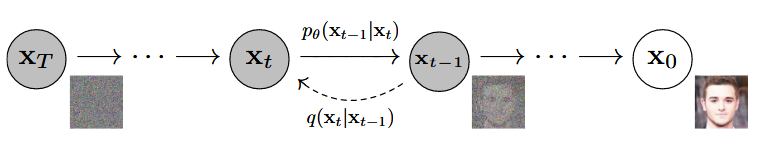
\includegraphics[width=0.6\textwidth]{imgs/ho_diffusion_process.png}
    \caption{Illustration of the diffusion process}
    \label{img:diff}
\end{figure}
DDPM, presented in \cite{hoDenoisingDiffusionProbabilistic2020}, is a solution to the problem presented above.  The main idea, presented on \cref{img:diff}, is to build  for any $x_0 \in \mathcal{X}$ a sequence $(x_t)_{0 \leq t \leq T}$ such that for any $t \in \llbracket 2; T\rrbracket$, $x_{t}$ is obtained from $x_{t-1}$ by adding a Gaussian noice to it: $\mathcal{N}(x_{t+1}; \sqrt{1 - \beta_t} x_t, \beta_t I)$, where $(\beta_t)_{1 \leq t \leq T}$ is a fixed sequences to be fixed. Using this process, rather than learning to generate an element of $\mathcal{X}$ from a white noise, they learn a model $p_\theta$ that given $(x_t,t)$ learns to predict $x_{t-1}$. They parametrisze $p_\theta$ to be $\mathcal{N}(x_{t-1}; \mu_\theta(x_t,t),\Sigma_\theta(x_t,t))$ and fixed $\Sigma_\theta$ to a constant to ease the computations.  Using maths and $\Sigma_\theta$ constant, they found that they can just learn $\epsilon$ (the noise added from $x_{t-1}$ to $x_t$) and optimize the loss (where $\alpha_t = 1 - \beta_t$, $\bar{\alpha_t} = \prod_{i=0}^t \alpha_i, {\beta_t} = \prod_{i=0}^t \beta_i$):
\begin{align}
    E_q \left[ \frac{\beta_t^2}{2 \sigma_t^2 \alpha_t (1 - \bar{\alpha_t})} \|\epsilon - \epsilon_\theta (\sqrt{\bar{\alpha_t}} x_0 + \sqrt{1 - \bar{\alpha_t}} \epsilon, t)\|\right] \label{eq:loss1}
\end{align}

\begin{figure}[h]
    \centering
    \begin{minipage}[b]{0.3\textwidth}
        \centering
        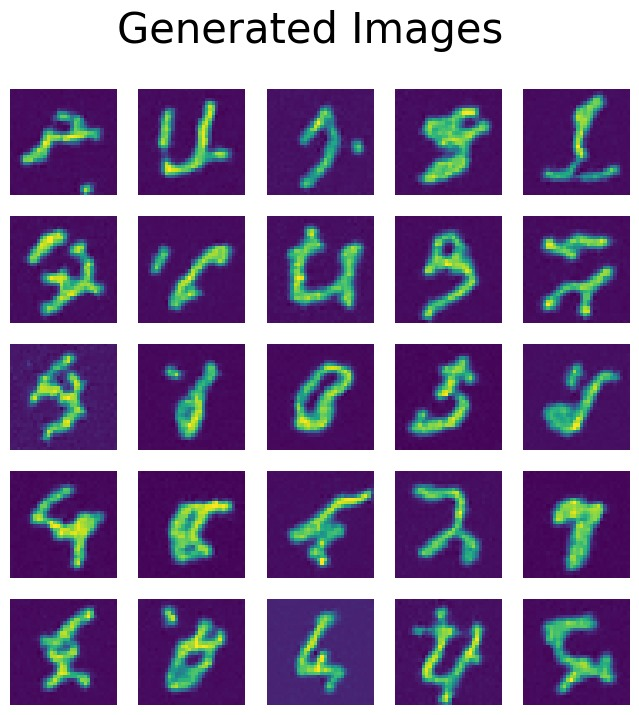
\includegraphics[width=\textwidth]{imgs/mnist_res.jpg}
        \caption{Our generation of hand-written digits}
        \label{img:ourresults}
    \end{minipage}
    \hfill
    \begin{minipage}[b]{0.65\textwidth}
        \centering
        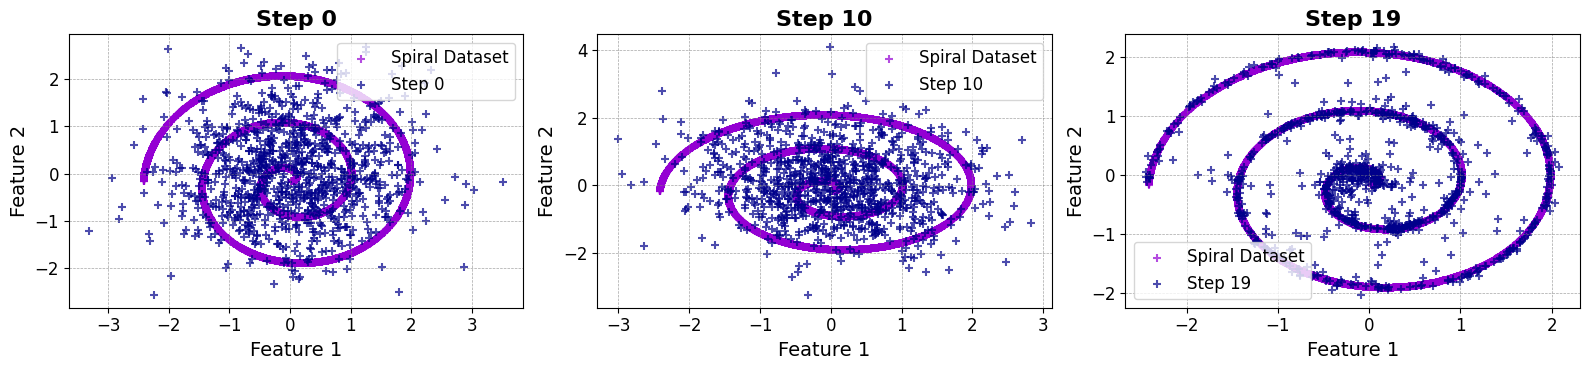
\includegraphics[width=\textwidth]{imgs/res_spirale.png}
        \caption{Diffusion visualization on Spirale}
        \label{img:spiralresults}
    \end{minipage}
\end{figure}


We have implemented (https://github.com/crdevio/DiffusionModel) this model, based on the code of Dataflowr (Marc Lelarge), and tested it on three distributions: Gaussian, Spirale, and MNIST. One can see on \cref{img:ourresults} our generation of hand-written digits and on \cref{img:spiralresults} a visualization of our diffusion implementation.

\section{Ameliorations}

Some datasets need a $T >> 1000$ to perform well, but you may want to have a trade-off between quality and cost of generation. An easy trick is to see that our model is learning to generate $\epsilon_t$ such that $x_t = x_0 + \sigma_{t,0} \epsilon_t$ (reparametrization trick in \cite{hoDenoisingDiffusionProbabilistic2020}). From this equation, one can get an approximation of $x_0$, $\tilde{x_0} = x_t - \sigma_{t,0} \epsilon_t$ and generate $\tilde{x}_{t-k} = \tilde{x_0} + \epsilon_{t-k}$.  Hence, by fixing $k \geq 1$ one can generate an image in $T/k$ steps.

In \cite{nicholImprovedDenoisingDiffusion2021} and \cite{dhariwalDiffusionModelsBeat2021}, OpenAI explored many upgrades to the standard DDPM, one of the main ideas is to let $\Sigma_\theta$ be learned between $\beta_t$ and $\tilde{\beta_t}$ (the two limits found by \cite{hoDenoisingDiffusionProbabilistic2020}).

Diffusion was proposed as a replacement for GANs (though GANs are still used, as witnessed by the Test of Time award from NeurIps) and GANs have access to labeled data to train. Hence, in \cite{dhariwalDiffusionModelsBeat2021}, labels were used to train Diffusion models. The idea is to sample according to a Gaussian that now also depends on $\nabla \log p (y \mid x_t)$ where $y$ is the desired label. The intuition behind that comes from Langevin Dynamics, which allows one to do a Markov process depending on $\nabla \log p(x)$ to sample from $p(x)$ without knowing $p(x)$. Here, a pre-trained classifier can estimate $\nabla \log p(x)$. However, for some data it is too hard to train a classifier, hence \cite{hoClassifierFreeDiffusionGuidance2022} introduces a classifier-free guidance that can perform the same results without needing a classifier, it relies on training simultaneously, two diffusion models, one that knows the label of data and one that does not.

Using the building block of classifier-free guidance, OpenAI introduced CLIP \cite{radford2021learningtransferablevisualmodels} that don't take labels as input but prompts. The main idea is to replace the label with a vector of representation (it is called Representation Learning, \cite{bengio2014representationlearningreviewnew}) and to also have a model that takes an image andreturnsn a vector of the same dimension. Then they train a model to give the distance between two learned vectors, and they use its gradient to direct the image generation to a prompt.

State-of-the-art models, such as ControlNet \cite{zhangAddingConditionalControl2023} accept more inputs, such as sketch, or canye edges to draw from.




\printbibliography % Afficher la bibliographie

\end{document}
